\documentclass[10pt,a4paper]{article}

\usepackage[latin1]{inputenc}
\usepackage{amsmath}
\usepackage{amsfonts}
\usepackage{amssymb}
\usepackage{graphicx}
\usepackage{listings}
\title{Assignment No :A1}
\date{}

\begin{document}
\maketitle
\section{Title:}
Divide and conquer.

\section{Problem Definition}
Using Divide and Conquer Strategies and object-oriented software design
technique using Modelio to design a software function for Binary Search for an
un-ordered data stored in memory. Use necessary USE-CASE diagrams and
justify its use with the help of mathematical modeling and related efficiency.
Implement the design using Eclipse C++ or python.

\section{Learning Objectives}
\begin{enumerate}
\item To study binary search algorithm.
\item To model the system using Use Case and Class Diagram.
\item To perform problem decomposition using divide and conquer method.
\end{enumerate}

\section{Learning Outcomes}
\begin{enumerate}
\item Ability to analyze problems as search.
\item Understanding of problem solving using divide and conquer strategies.
\item Profound knowledge of documenting a software system.
\end{enumerate}


\section{Related Mathematics}
Let S be the solution perspective of the given problem.\\
The set S is defined as:\\\\
$S=\lbrace\ s,e,X,Y,F,DD,NDD,S_{c},F_{c}|\varnothing_{s}\rbrace$ \\
Where,

s= Start state,  Such that $Y=\lbrace \varnothing \rbrace$ 

e= End state  \\\\
X= Input Set. \\\\
$X=\lbrace$ seq(x) $\mid$ x $\in$ NN (natural numbers) $\rbrace$ \\
Where,

NN $\in \lbrace$ Positive Integers $\rbrace$ - 0 *and* seq in sorted order\\\\ 
Y=Output set.\\
$Y=\lbrace$ search index $\rbrace $ \\\\
F= Set of functions used.\\
F=$\lbrace divide(), check(), conquer() \rbrace$ \\\\
divide() = function to divide the list in two halves\\
check() = function that checks the half to be searched next\\
conquer() = recursive call the function searching half list\\\\
DD=Deterministic data. \\
DD=
\begin{enumerate}
\item input sequence in sorted order.
\item search element exists in the sorted order.
\item search terminates. (list is finite)\\\\
\end{enumerate}
NDD= Non-deterministic data. \\
\\NDD= $\cup$ - DD\\


\section{State Transition diagram}
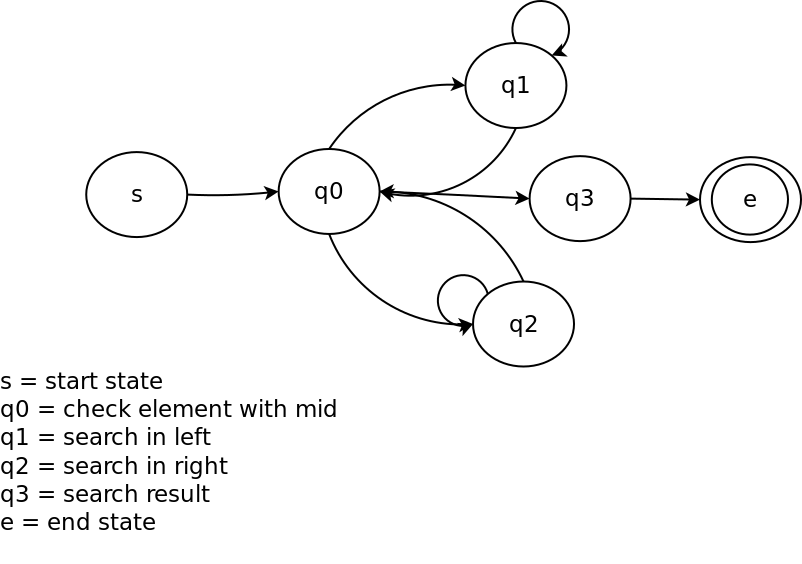
\includegraphics[scale=0.35]{stdg.png}

\newpage
\section{Concepts related theory}
In computer science, divide and conquer (D and C) is an algorithm design paradigm based on multi-branched recursion. A divide and conquer algorithm works by recursively breaking down a problem into two or more sub-problems of the same or related type, until these become simple enough to be solved directly. The solutions to the sub-problems are then combined to give a solution to the original problem.

This divide and conquer technique is the basis of efficient algorithms for all kinds of problems, such as sorting (e.g., quicksort, merge sort), multiplying large numbers (e.g. the Karatsuba algorithm), finding the closest pair of points, syntactic analysis (e.g., top-down parsers), and computing the discrete Fourier transform (FFTs).

Understanding and designing D and C algorithms is a complex skill that requires a good understanding of the nature of the underlying problem to be solved. As when proving a theorem by induction, it is often necessary to replace the original problem with a more general or complicated problem in order to initialize the recursion, and there is no systematic method for finding the proper generalization. These D and C complications are seen when optimizing the calculation of a Fibonacci number with efficient double recursion.

The correctness of a divide and conquer algorithm is usually proved by mathematical induction, and its computational cost is often determined by solving recurrence relations.

\section{Use Case Diagram}
	\begin{figure}[h!]
		\centering
		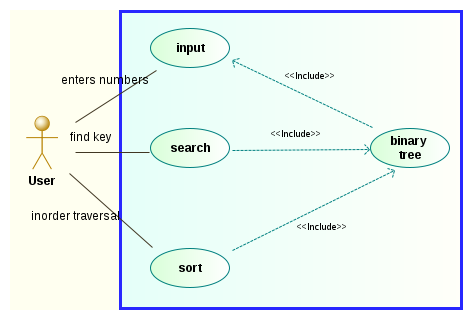
\includegraphics[scale=0.50]{use_case_diagram.png}
		\caption{Use Case Diagram}
		\label{Use Case Diagram}
	\end{figure}

\newpage
\section{Class Diagram}
\begin{figure}[htb!]
		\centering
		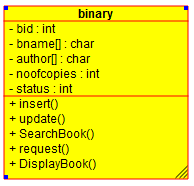
\includegraphics[scale = 0.80]{bst-class}
		\caption{Class Diagram}
		\label{Class Diagram}
		\end{figure}

\section{Program Listing}
\begin{lstlisting}
//============================================================================
// Name        : main.py
// Author      : ANIMESH_K
// Version     : 3.0
// Copyright   : all rights reserved
// Description : Assignment_A1 for CL3
//============================================================================

theta = u'\u0398'
def makeAList(s):
    return map(int, s.split(' '))
def take_input():
    print "Please enter the elements separated by space"
    input_array = raw_input().split(' ')
    return map(int, input_array)
class Node:
    def __init__(self, data=-1, left = None, right=None):
        self.right = right
        self.left = left
        self.data = data
    def __str__(self):
        s = ""
        if self.left != None:
            s = s+ str(self.left.data)+"<--"
        s = s + "|"+str(self.data)+"|"
        if self.right!=None:
            s = s+ "-->"+str(self.right.data)
        #return "."+s+"."
        return s

class BinarySearchTree:
    def __init__(self):
        self.root = None
    def populateTree(self):
        input_array = take_input()
        #input_array = makeAList("4 3 6 1 2 5 7")
        for element in input_array:
            self.addElement(element)
    def addElement(self, element):
        if self.root == None:
            # this is the first element
            self.root = Node(element)
        else:
            # now find the parent here.
            parent = self.findParent(element)
            if parent != None:
                # now make the new node here
                newNode = Node(element)
                if element > parent.data:
                    parent.right = newNode
                else:
                    parent.left = newNode
            else:
                print "element already exists, cannot insert the new element"
    def inorderTraversal(self):
        if self.root == None:
            print "tree empty!"
            return
        self.inorder(self.root)
        print ""
    def inorder(self, node):
        if node == None:
            return
        self.inorder(node.left)
        print node,
        print " ",
        self.inorder(node.right)
    def findParent(self, element):
        '''
        this function returns the possible parent of 
        the new element to be inserted
        it will return None if element already exists
        Note: root is not None
        '''
        current = self.root
        parent = current
        while current!=None:
            parent = current
            if element > current.data:
                current = current.right
            elif element < current.data:
                current = current.left
            else:
                return None
        return parent
    def showMenu(self):
        menu = ["add a new element", "search for an element", "sort", "exit"]
        while True:
            for i in range(len(menu)):
                print str(i+1)+". "+menu[i]
            print ">>>",
            choice = int(raw_input())
            if choice == 1:
                element = int(raw_input("Enter the element to be added: "))
                self.addElement(element)
                self.printComplexity()
            elif choice==2:
                element = int(raw_input("Enter the element to be searched: "))
                res = self.findParent(element)
                if res == None:
                    print "Found"
                    self.printComplexity()
                else:
                    print "Not found!"
            elif choice==3:
                self.inorderTraversal()
                print "Average case: "+theta+"(n)"
            elif choice==4:
                break
            else:
                print "wrong input!"
    def printComplexity(self):
        print "Worst case: "+theta+"(n)"
        print "Best case: "+theta+"(log n)"
        
        

def main():
    tree = BinarySearchTree()
    tree.populateTree()
    tree.showMenu()
    print "The program will now exit"
main()

\end{lstlisting}


\section{Output}
\begin{lstlisting}

Please enter the elements separated by space
1 2 3 4 5 6 7 8 9 10 11 12 13 14 15 
1. add a new element
2. search for an element
3. sort
4. exit
>>> 2
Enter the element to be searched: 5
Found
Worst case: \u0398(n)
Best case: \u0398(log n)
1. add a new element
2. search for an element
3. sort
4. exit
>>> 1
Enter the element to be added: 20
Worst case: \u0398(n)
Best case: \u0398(log n)
1. add a new element
2. search for an element
3. sort
4. exit
>>> 3
|1|-->2   |2|-->3   |3|-->4   |4|-->5   |5|-->6   |6|-->7   |7|-->8   |8|-->9   |9|-->10   |10|-->11   |11|-->12   |12|-->13   |13|-->14   |14|-->15   |15|-->20   |20|   
Average case: \u0398(n)
1. add a new element
2. search for an element
3. sort
4. exit
>>> 4
The program will now exit

\end{lstlisting}

\section{Testing}
\subsection{Black box testing}
Black-box testing is a method of software testing that examines the func-
tionality of an application based on the specifications. It is also known as
Specifications based testing. Independent Testing Team usually performs
this type of testing during the software testing life cycle.This method of test
can be applied to each and every level of software testing such as unit, inte-
gration, system and acceptance testing.
Black box testing techniques are :

\begin{enumerate}
	\item Equivalence Class Partitioning
	\item Boundary Value Analysis
	\item Decision Tables
	\item State Transition Diagrams (or) State	Transition Diagrams
	\item Orthogonal Arrays
	\item All Pairs Technique
\end{enumerate}


\subsection{White box testing}
		 White Box Testing (WBT) is also known as Code-Based Testing or Structural Testing. White box testing is the software testing method in which internal structure is being known to tester who is going to test the software. In this method of testing the testcases are calculated based on analysis internal structure of the system based on Code coverage, branches coverage, paths coverage, condition Coverage etc. Typically such method are used at Unit Testing of the code but this different as Unit testing done by the developer \& White Box Testing done by the testers, this is learning the part of the code \& finding out the weakness in the software program under test.
For tester to test the software application under test is like a white/transparent box where the inside of the box is clearly seen to the tester (as tester is aware/access of the internal structure of the code), so this method is called as White Box Testing.

The White-box testing is one of the best method to find out the errors in the software application in early stage of software development life cycle. In this process the deriving the test cases is most important part. The test case design strategy include such that all lines of the source code will be executed at least once or all available functions are executed to complete 100 percent  code coverage of testing. For this, we will use Flow Graphs. Flow graphs are, Syntactic abstraction of source code Resembling to classical flow charts Forms the basis for white box test case generation principles.Conventions of flow graph notation. \\
Why and When White-Box Testing:\\
White box testing is mainly used for detecting logical errors in the program code. It is used for
debugging a code, finding random typographical errors, and uncovering incorrect programming
assumptions .
White box testing is done at low level design and implementable code. It can be applied at all levels of
system development especially Unit, system and integration testing. White box testing can be used for
other development artefacts like requirements analysis, designing and test cases .
White box testing techniques are:\\
1. Static white box testing\\
a. Desk checking\\
b. Code walkthrough\\
c. Formal Inspections\\
2. Structural White box testing\\
a. Control flow/ Coverage testing\\
b. Basic path testing\\
c. Loop testing\\
d. Data flow \\


Sample Input: For integer array int A[] = 1,2,3,4,5,6,7,8,9,10; Function 
is passed\\
following arguments: Binary Search(A, 1, 10, 7);\\
Output obtained: Entered second Entered third Entered first 6\\
The underlined nodes are the ones being tested. The above output shows
that every test region is covered for given input.\\
\begin{figure}[h!]
	\centering
	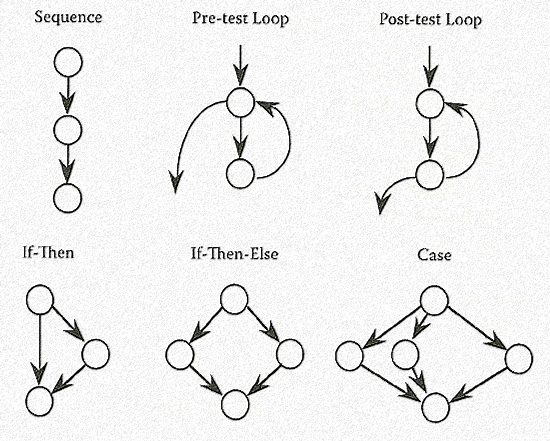
\includegraphics[scale=0.30]{CFG.png}
\end{figure}

\subsection{ POSITIVE/NEGATIVE TESTING }

\textbf{Positive Testing :}\\
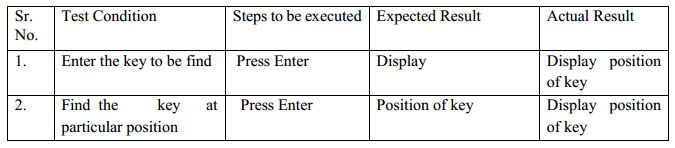
\includegraphics[width=\textwidth]{binary_positive}
\vspace{30px}

\textbf{Negative Testing :}\\
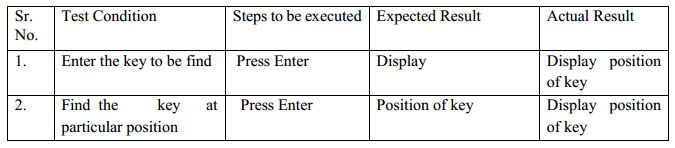
\includegraphics[width=\textwidth]{binary_positive}

\section{Conclusion}
Thus we have studied divide and conquer method and implemented binary search on unordered natural numbers in python. We have also acquired an acute understanding of exemplary documentation used in software design.

\end{document}